\documentclass[main.tex]{subfiles}

\begin{document}

\section{\starpu} \label{chapter:starpu}

\starpu \cite{augonnet2011starpu} is a unified runtime system consisting on both software and a runtime API that aims to allow programmers of computational intensive applications to more easily exploit the power of available devices, supporting \cpus and \gpus.

Much like \gama, this framework frees the programmer of the workload scheduling and data consistency inherent from a \hetplat. Task submissions are handled by the \starpu task scheduler, and data consistency is ensured via a data management library.

However, one of the main differences comes from the fact that \starpu attempts to increase performance by carefully considering and attempting to reduce memory transfer costs. This is one by using history information for each task and, accordingly to the scheduler's decision of where a task shall be executed, asynchronously prepare data dependencies, while the system is busy computing other tasks. The task scheduler itself can take this into account, and determine where a task should be executed by taking into account not only execution history, but also the estimation of data transfers latency.

\subsection{Terminology}

\starpu uses a well defined terminology to describe its libraries and API:

\begin{description}
  \item[Data Handle] \hfill \\
    References a memory block. The allocation of the required space, and the possibly required memory transfers to deliver information to each device can be completely handled by \starpu;

  \item[Codelet] \hfill \\
    Describes a computational kernel that can be implemented in one or more architectures, such as \cpus, \cuda or \acs{OpenCL}. It also stores information about thew amount and type of data buffers it should receive;

  \item[Task] \hfill \\
    Is defined as the association between a codelet and a set of data handles;

  \item[Partition] \hfill \\
    The subdivision of a data handle in smaller chunks, according to a partitioning function, which can be user defined;

  \item[Worker] \hfill \\
    A processing element, such as a \cpu core, managed by StarPU to execute tasks;

  \item[Scheduler] \hfill \\
    The library in charge of assigning tasks to workers, based on a well defined scheduling policy.

\end{description}

\subsection{Task Scheduling}

The framework employs a task based programming model. Computational kernels must be encapsulated within a task. A given kernel can be implemented in multiple ways (i.e. for \cpus or for \cuda), and \starpu will handle the decision of where and when the task should be executed, based on a task scheduling policy.

Data manipulated by a task is automatically transferred as needed between the various processing devices, ensuring memory consistency and freeing the programmer from dealing directly with scheduling issues, data transfers and other requirements associated with it.

Previous work by the \starpu development team indicates that one of the most important issues with scheduling is about obtaining an accurate performance model for the execution time of a task \cite{augonnet2010data,augonnet2010automatic}. This is increasingly difficult when data transfers, which the team regards as a key issue, are taken into account, as shown in the latter paper. In it, a data-prefetching implementation for \gpus is present, and asynchronous data request capability is introduced as part of the \starpu library, with the goal of preventing computational units from being stalled waiting for data.

\subsection{Dependencies}

\starpu automatically builds a dependency graph of all submitted tasks, and keeps them in a pool of \emph{frozen tasks}, passing them onto the scheduler once all dependencies are met.

Dependencies can be implicitly given by the data manipulated by the task. Each task receives a set of buffers, each one corresponding to a piece of data managed by \starpu data management library, and will wait until all the buffers from which it must read are ready.

This includes the possible data transfers that are required to meet dependencies, in case different tasks that depend on the same data are scheduled to run on different computational nodes. \starpu will automatically make sure the required data transfers are made between each task execution to ensure data consistency.

In addition to implicit data dependencies, other dependencies can be explicitly given in order to explicitly force the execution order of a given set of tasks.

\subsubsection{Data Access Modes} \label{sec:starpu:data_access}

Each data dependency that is explicitly defined in a task can have a different access mode. Data can be used in read-only, write-only or read-write mode. This access mode does not serve the purpose of ensuring memory correctness. It is used to soften task dependencies by using a \emph{Multiple Readers / Single Writer} model in dependency calculation.

This model describes a type of mutual exclusion pattern where a data block can be concurrently accessed by any number of reader, but must be exclusively accessed by a writer. \starpu uses this concept to further optimize data dependency calculations. If multiple scheduled tasks depend on the same data handle, but only with reading access, then that dependency should not block the multiple tasks from running concurrently (see \cref{fig:starpu_dep}. Temporary copies of the data can be created, possibly on different computational units, and later discarded immediately, since a read-only buffer is assumed to remain unchanged at the end of a task.

\begin{figure}[!htp]
  \centering
  \begin{subfigure}{.5\textwidth}
    \centering
    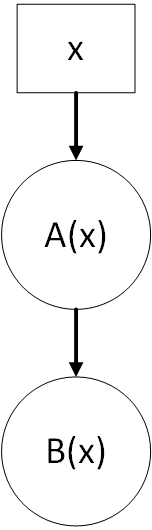
\includegraphics[width=0.2\linewidth]{visio/starpu_dep_rw}
    \caption{Since A writes to $x$, B must wait for it to finish to solve the dependency \label{fig:starpu_dep_rw}}
  \end{subfigure}%
  \begin{subfigure}{.5\textwidth}
    \centering
    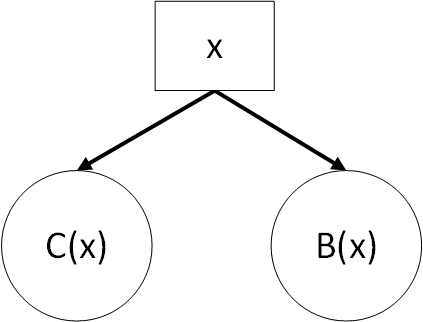
\includegraphics[width=0.6\linewidth]{visio/starpu_dep_r}
    \caption{Neither B nor C write to $x$, so they can be ran concurrently \label{fig:starpu_dep_r}}
  \end{subfigure}
  \caption{Access mode illustration. Task A requires read/write access to $x$, while tasks B and C require read-only access \label{fig:starpu_dep}}
\end{figure}

\subsection{Virtual Shared Memory}

The approach used by \starpu when it comes to memory management is simpler than the model employed by \gama. The purpose is the same: to automatically manage memory allocations and transfers on all devices. This not only frees the programmer from the work of manually managing memory between tasks, but it also has the potential to lower the cost of such operations.
\starpu manages memory by forcing the user to declare data handles to their data. These handles are used as arguments for tasks, allowing the scheduler to allocate and transfer all required data buffers to the correct computational unit prior to the task execution.

\subsection{Multi-threading} \label{section:starpu_multithreading}

In order to have an accurate view of the topology of the system, the framework can optionally use the \texttt{hwloc} library\footnote{\texttt{hwloc}, or Portable Hardware Locality, is a package that provides access to an abstract topology of modern computational architectures.} \cite{broquedis2010hwloc} to detect the structure of the architecture, including all \cpu sockets, \acs{NUMA} nodes and cache hierarchy.

A tree is created representing the complete hierarchy of the system. Latest version of the framework also introduce support for parallel tasks, with the concept of combined workers. These workers exist in cases where the system has multiple computational units in the same node (such as \cpu sockets where multiple cores share a cache hierarchy). In these situations, and if \starpu is using a parallel-task-aware scheduler (currently only \texttt{pheft} and \texttt{peager} exist), it is possible to specify the maximum degree of parallelism for a function. A combined worker can then be assigned to such tasks using, for example, \openmp to take advantage of the multiple available cores.

\subsection{API} \label{section:starpu_api}

Two API versions are made available. The high-level, \texttt{pragma}-based\footnote{Directives inserted within the code, to instruct the compiler about how to process input. Can be used to extend the compiler and provide additional features, functionality or optimizations} API. This exposes \starpu's main functionality with a set of directives that can be added to the code in order to embed \starpu within it. It is particularly suited for less experienced developers, or developers who simply need to focus completely in the algorithmic issues with less or no knowledge about the underlying parallel hardware being used underneath.

The directives can be easily disabled, restoring the application to its original, \starpu-free nature, which also makes it ideal to add \starpu into already existing code, or applications that require a large degree of portability.

The low-level version is a more verbose one, which is actually used internally by the high-level one, and provides a greater degree of control over what \starpu does.

This trade-off is not uncommon, with many existing libraries besides \starpu supporting both API levels. High level versions are designed to remove complexity and accelerate development time. They are often a subset of an underlying low level version, delivering only the more common features. More experienced developers should be able to achieve better results with a lower level API, with the cost of additional development time.

\subsection{Performance Model}

Most schedulers available with \starpu are history based. This relies on the programmer to configure a performance model for each defined codelet, in order to allow the framework to identify it, and use on-line calibration. Calibration results will be stored in a centralized directory, and inform \starpu about how each codelet behaves on each different device, with a certain input size.

Once a good calibration has been obtained (with a minimum number of executions of a task), \starpu can schedule tasks more efficiently, according to the policy defined by the scheduler. The list of the available scheduling policies is the following:

\begin{description}

\item[eager] The default scheduler, using a single task queue, from which workers draw tasks. This method does not allow to take advantage of asynchronous data prefetching, since the assignment of a task is only done when a given worker requires so;

\item[prio] Similar to eager, but tasks can be sorted by a priority number;

\item[random] Tasks are distributed randomly, according to the estimated performance of each worker. Although extremely naive, this has the advantage of allowing data prefetching, and minimizing scheduler decision times;

\item[ws (Work Stealing)] Once a worker becomes idle, it steals a task from the most loaded worker

\item[dm (Deque Model)] Performs a HEFT-like strategy, similarly to \gama (see \cref{sec:gama_sched}). Each task is assigned to where the scheduler thinks its termination time will be minimized;

\item[dmda (Deque Model Data Aware)] Similar to \textbf{dm}, but also taking into account data transfer times;

\item[dmdar (Deque Model Data Aware Ready)] Similar to \textbf{dmda}, but tasks are sorted per-worker, based on the amount of already available data buffers for that worker. Devices where most or all data buffers a task depends on are more likely to receive that task, in order to attempt minimization of data transfers;

\item[pheft (parallel HEFT)] similar to \textbf{heft} (which is deprecated in \starpu, with \textbf{dmda} working in a very similar way), with support for parallel tasks

\item[peager] similar to \textbf{eager}, with support for parallel tasks

\end{description}

Additionally, schedulers are built as a pluggable system, allowing developers to write their own scheduling policies if desired, and easily use them within \starpu.


\subsection{Task Granularity}

The granularity of a task in \gama can be automatically defined and readjusted with the use of a dicing function, that recursively adjusts it to find the best case scenario for each particular device. This feature is not available in \starpu, where granularity has to be defined manually by the programmer.

The API gives the ability to subdivide a data handle into smaller children, based on a partitioning function. This partitioning can be defined as a simple vector or matrix block partitioning, but more complex and custom methods can be defined.

After partitioning, each children can be used as a different data handle. This means that in order to operate in chunks of data at a time, one has to first partition data according to a user defined policy, and later submit multiple individual tasks, using each child data handle individually.

\end{document}


